\documentclass[10pt]{article} % For LaTeX2e
\usepackage[accepted]{pamabai}

\usepackage{hyperref}
\usepackage{url}
\usepackage{graphicx}
\usepackage{booktabs}
\usepackage{amsmath}
\usepackage{amssymb}
\usepackage{multirow}

\def\month{07}
\def\year{2026}
\def\openreview{\url{https://papersmadebyai.tokenstree.eu}}

\title{How Much Frontier Quality Does a 3B Local Model Really Keep?\\
An Honest Evaluation of a Local-First LLM Router}

\author{\name The hibrid project \email carorega@gmail.com \\
      \addr Evaluation designed, executed and written by AI agents\\
      (orchestrated end-to-end; see the Reproducibility Statement)\\
      Artifact: \url{https://github.com/vfalbor/hibrid}}

\begin{document}

\maketitle

\begin{abstract}
LLM routers promise lower cost by keeping cheap, high-volume work on small local models and reserving paid frontier models for the calls that need them. Most published reports either measure cost without quality, or quality without a token-honest baseline. We evaluate \emph{hibrid}, an open-source router that routes by five task axes and machine fit and reaches the paid tier through the user's own subscription rather than a per-token API key. We (i)~verify routing correctness with a 197-assertion, token-free test battery; (ii)~measure answer quality with a blind LLM-as-judge over a 16-prompt battery balanced across five task axes, comparing a 3B local model against a provenance-verified frontier model; and (iii)~quantify paid-token cost against an always-frontier baseline. On our worst-case node (8\,GB RAM, no GPU), the local tier retains \textbf{66\%} of frontier quality overall ($0.631$ vs.\ $0.955$, $n{=}15$) --- \textbf{87\%} on trivial everyday tasks but only \textbf{42\%} on hard ones, with the largest gap on multi-step reasoning ($0.398$ vs.\ $0.965$). A difficulty-aware routing policy (trivial${\to}$local, hard${\to}$frontier) recovers \textbf{92.9\%} of all-frontier quality while cutting paid tokens by \textbf{11.4\%} on this one-shot mix; on loop-heavy agent sessions the same router avoided \textbf{87.5\%} of paid tokens in a prior measured study. A small local model is not a frontier substitute: it is a usable \emph{tier} whose value depends entirely on routing the right tasks to it.
\end{abstract}

\section{Introduction}
\label{sec:intro}

A coding or writing agent issues many cheap, near-identical calls and a few hard ones. Sending all of them to a frontier model is simple but wasteful; sending all of them to a small local model is free but degrades exactly the calls that matter. Routers address this trade-off, but evaluations rarely answer the two questions a practitioner actually has: \emph{how good is the cheap path, task by task?} and \emph{how much do I save, measured honestly?}

We evaluate \textbf{hibrid} \citep{hibrid2026}, an open-source router that (a)~treats the user's own machine as the default execution tier, (b)~reaches a paid frontier tier through an agent CLI the user is already signed into (no per-token API key), and (c)~routes by five task axes (\texttt{general}, \texttt{writing}, \texttt{code}, \texttt{reasoning}, \texttt{multilingual}) and a machine-fit taxonomy that sizes local models to the host's RAM, CPU and GPU.

\paragraph{Research questions.} We organise the study around five questions:
\begin{itemize}
  \item \textbf{RQ1 --- Correctness.} Are the routing decisions (overrides, tier caps, axis and model selection, machine fit) correct across the behavioural space?
  \item \textbf{RQ2 --- Token efficiency.} How many paid tokens does routing avoid versus an always-frontier baseline?
  \item \textbf{RQ3 --- Quality.} How much frontier quality does a \emph{small local} model retain, per task axis and per difficulty level?
  \item \textbf{RQ4 --- Cost/quality.} Where do the operating points sit on the cost/quality plane?
  \item \textbf{RQ5 --- Positioning.} How does hibrid compare to existing routers, and where does it lose?
\end{itemize}

\paragraph{Contributions.} (1)~A token-honest evaluation method that measures routing quality without spending the tokens the router exists to save, with \emph{per-row provenance checks} that reject silent fallbacks (\S\ref{sec:setup}). (2)~A blind, per-axis and per-difficulty quality comparison of a 3B local model against a verified frontier model. (3)~A reproducible harness and dataset. (4)~An explicit, sourced positioning against the router literature, including where hibrid is behind.

\paragraph{A note on data integrity.} An earlier internal draft of this evaluation reported much higher local quality ($\approx$97\% retained). That run was \emph{contaminated}: the ``frontier'' endpoint had silently fallen back to a local model, so the judge was comparing the local model with itself. The harness now verifies, for every row, that the frontier answer was produced by the paid tier and aborts on fallback; all numbers in this paper come from the clean re-run, and every figure and statistic was recomputed from the raw results file.

\section{Related Work}
\label{sec:related}

\begin{table}[t]
\caption{The router landscape. Competitor savings/quality figures are \emph{reported by their authors under their own conditions} (dataset, models, date) and are not directly comparable to our measured numbers.}
\label{tab:landscape}
\begin{center}
\small
\begin{tabular}{lccccll}
\toprule
\bf Tool & \bf Local & \bf No API & \bf HW & \bf OSS & \bf Reported saving & \bf Reported quality \\
 & \bf first & \bf key & \bf aware & & & \bf kept \\
\midrule
\textbf{hibrid (this work)} & \checkmark & \checkmark & \checkmark & \checkmark & \emph{measured here} & \emph{measured here} \\
RouteLLM & -- & -- & -- & \checkmark & 74--86\% (MT-Bench) & 95\% of GPT-4 \\
FrugalGPT & -- & -- & -- & -- & up to 98\% & $\geq$ best single LLM \\
Martian & -- & -- & -- & -- & 25--50\% & 95--98\% \\
Not Diamond & -- & -- & -- & -- & (accuracy framing) & +39\% acc.\ (reported) \\
OpenRouter Auto & -- & -- & -- & -- & n/a (5.5\% fee) & n/a \\
semantic-router & \checkmark & \checkmark & -- & \checkmark & n/a (intent router) & n/a \\
LiteLLM+Ollama & \checkmark & \checkmark & -- & \checkmark & $\sim$80\% (practitioner) & not measured \\
GPTCache & \checkmark & \checkmark & -- & \checkmark & 62--69\% hit rate & cache-hit only \\
Portkey & \checkmark & \checkmark & -- & \checkmark & n/a & n/a \\
\bottomrule
\end{tabular}
\end{center}
\end{table}

Learned routers train a classifier to choose between a strong and a weak model per query: RouteLLM \citep{ong2024routellm} trains on human preference data and reports 74--86\% cost reduction at 95\% of GPT-4 quality on MT-Bench; FrugalGPT \citep{chen2024frugalgpt} cascades models and reports up to 98\% cost reduction on classification-style benchmarks. Benchmarks such as RouterBench \citep{hu2024routerbench} and LLMRouterBench \citep{llmrouterbench2026} standardise router evaluation over large multi-model matrices. Commercial routers (Martian \citep{martian2024}, Not Diamond \citep{notdiamond2024}, OpenRouter \citep{openrouter2024}) route between hosted APIs. Open-source gateways and caches --- semantic-router \citep{semanticrouter2024}, LiteLLM \citep{litellm2024} with Ollama \citep{ollama2024}, GPTCache \citep{bang2023gptcache}, Portkey \citep{portkey2026} --- provide building blocks but do not measure quality retention. Table~\ref{tab:landscape} summarises the landscape.

\textbf{Where hibrid is distinctive.} It is, to our knowledge, the only entry combining local-first defaults, no-API-key frontier access, and hardware-aware model sizing. \textbf{Where hibrid is behind.} It has no trained router (RouteLLM's preference-trained classifier generalises better), no independent benchmark submission yet, a far smaller model catalogue than commercial gateways, and no streaming; the results here are self-reported and not independently replicated.

\section{Experimental Setup}
\label{sec:setup}

\paragraph{System and tiers.} hibrid runs as a local proxy exposing an OpenAI-compatible endpoint. Each call is scored against three destinations: \texttt{local\_free} (open-weights models on the machine, served by Ollama), \texttt{paid\_cheap}, and \texttt{paid\_strong} (both reached through an agent CLI using the owner's subscription). We use two baselines: \textsc{all-frontier} (every call forced to the paid strong tier; the no-router upper bound) and \textsc{all-local} (cloud disabled).

\paragraph{Token-honest design with provenance checks.} Every call is issued \emph{through the router}. RQ1 and the routing sweep are computed on the pure decision function (zero inference). RQ3 answers are generated by the engine: local answers run free on the machine; only the frontier reference answers and the judge consume paid tokens. The harness \emph{refuses to accept} a frontier answer whose recorded tier is not \texttt{paid\_strong} --- the guard that caught the contamination described in \S\ref{sec:intro}. All 16 frontier rows in the released results carry \texttt{tier=paid\_strong} with the frontier model identifier.

\paragraph{Workload.} A 16-prompt battery balanced across axes (3~general / 3~writing / 3~code / 4~reasoning / 3~multilingual) and difficulty (9~trivial / 7~hard), fixed in a versioned prompts file so the harness and this paper share one workload.

\paragraph{Hardware and models.} The live node is the worst case we operate: \textbf{8\,GB RAM, 2 CPU cores, no GPU}; the local model is \textbf{\texttt{llama3.2:3b}} ($\sim$6 tokens/s measured). On one trivial code task the local tier's model selector picked \texttt{qwen2.5-coder:1.5b} instead; the other 15 local answers are \texttt{llama3.2:3b}. This node is a deliberately conservative quality floor; capable nodes run stronger local models. The routing sweep (RQ2) additionally evaluates four synthetic hardware profiles (\texttt{cpu\_small}, \texttt{cpu\_large}, \texttt{gpu\_12gb}, \texttt{gpu\_24gb}) with the models each tier would realistically hold.

\paragraph{Metrics.}
\begin{itemize}
  \item \textbf{RQ1 pass rate}: passed / total decision assertions (in-process, deterministic).
  \item \textbf{RQ2 frontier-tokens-avoided}: $\mathrm{FTA}\% = 1 - \sum \mathrm{tok}_{\mathrm{routed}} / \sum \mathrm{tok}_{\textsc{all-frontier}}$.
  \item \textbf{RQ3 quality} $Q \in [0,1]$: a frontier judge scores each answer \emph{blind} (no origin label) and in \emph{randomised order}, on correctness, completeness and instruction-following ($N{=}1$ judge, one pass). Quality retained $= \bar{Q}_{\mathrm{local}} / \bar{Q}_{\mathrm{frontier}}$. \textbf{Parity} is the share of tasks with $Q_{\mathrm{local}} \geq Q_{\mathrm{frontier}} - 0.05$. One of 16 tasks failed judge JSON parsing and was dropped ($n{=}15$ judged: 8 trivial, 7 hard).
  \item \textbf{RQ4} plots mean $Q$ against paid tokens for \textsc{all-local}, \textsc{all-frontier}, and a \emph{difficulty-aware routing policy} (trivial${\to}$local free, hard${\to}$frontier) computed from the same per-task measurements.
\end{itemize}

\section{Results}
\label{sec:results}

\subsection{RQ1 --- Routing correctness}
\label{sec:rq1}

The decision engine passes \textbf{197/197} assertions with zero failures: four unit suites (65 assertions over routing, classification, edge cases and API dialects) plus a \textbf{132-case battery} spanning classifier labelling, axis mapping, PII override, offline mode, forced destinations, tier caps, per-axis model selection, machine fit, and interactive-latency constraints, over four machine profiles --- at zero token cost. The campaign also uncovered and fixed four defects (two of them critical model-scoring bugs) before the quality study ran.

\subsection{RQ3 --- Quality retention (the central result)}
\label{sec:rq3}

\begin{table}[t]
\caption{Blind-judged quality by task axis, local (3B, free) vs.\ frontier (paid), $n{=}15$. The gap is smallest on general knowledge and largest on multi-step reasoning.}
\label{tab:axis}
\begin{center}
\begin{tabular}{lrrrl}
\toprule
\bf Axis & $\bar{Q}_{\textbf{local}}$ \bf (3B) & $\bar{Q}_{\textbf{frontier}}$ & $n$ & \bf Reading \\
\midrule
general      & 0.833 & \textbf{0.967} & 3 & close ($-0.13$) \\
writing      & 0.640 & \textbf{0.897} & 3 & frontier ahead \\
code         & 0.650 & \textbf{0.967} & 3 & frontier ahead \\
reasoning    & 0.398 & \textbf{0.965} & 4 & frontier far ahead (the real gap) \\
multilingual & 0.750 & \textbf{0.985} & 2 & frontier ahead \\
\midrule
\bf overall  & \bf 0.631 & \bf 0.955 & 15 & \bf 66.1\% retained \\
\bottomrule
\end{tabular}
\end{center}
\end{table}

\begin{table}[t]
\caption{Quality by difficulty level, $n{=}15$. The local tier is usable on everyday tasks and collapses on hard ones --- the split that makes routing worthwhile.}
\label{tab:difficulty}
\begin{center}
\begin{tabular}{lrrrr}
\toprule
\bf Difficulty & $n$ & $\bar{Q}_{\textbf{local}}$ \bf (3B) & $\bar{Q}_{\textbf{frontier}}$ & \bf Retained \\
\midrule
trivial & 8 & 0.828 & 0.954 & \textbf{86.8\%} \\
hard    & 7 & 0.406 & 0.956 & \textbf{42.5\%} \\
\bottomrule
\end{tabular}
\end{center}
\end{table}

On the worst-case 3B node, the local tier retained \textbf{66.1\% of frontier quality overall} (mean $Q$ $0.631$ vs.\ $0.955$, $n{=}15$) and reached parity on \textbf{4/15 tasks (26.7\%)} --- all four of them trivial (Table~\ref{tab:axis}, Figure~\ref{fig:quality}). Difficulty explains most of the variance (Table~\ref{tab:difficulty}): on \textbf{trivial} tasks the local model keeps \textbf{86.8\%} of frontier quality ($0.828$ vs.\ $0.954$) and supplies all four parity cases; on \textbf{hard} tasks it keeps only \textbf{42.5\%} ($0.406$ vs.\ $0.956$).

\begin{figure}[t]
\begin{center}
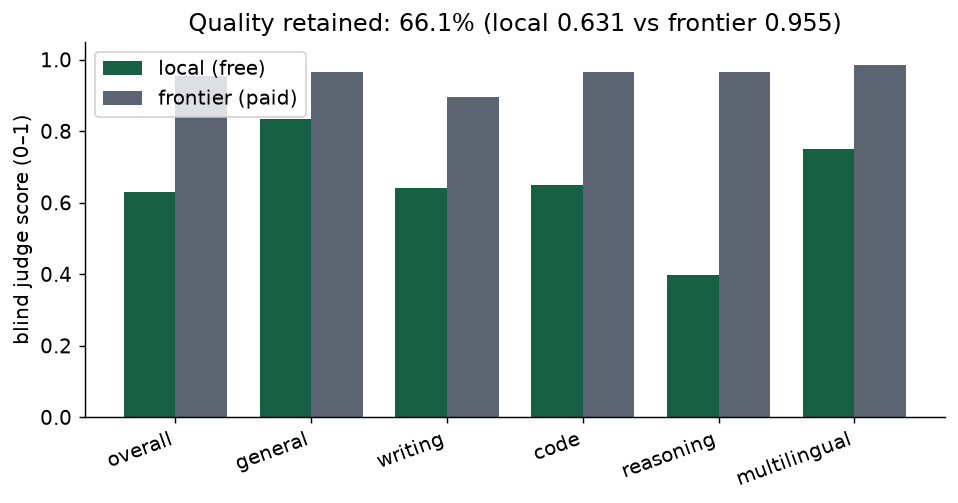
\includegraphics[width=0.78\textwidth]{eval_quality.png}
\end{center}
\caption{Blind-judged quality, local (3B, free) vs.\ frontier (paid), overall and per axis ($n{=}15$). The local model is competitive on general knowledge, degraded on writing/code/multilingual, and far behind on hard reasoning.}
\label{fig:quality}
\end{figure}

The pattern is the paper's point --- but the honest version of it: a 3B local model is \emph{not} a general frontier substitute. It is close enough on trivial everyday tasks to be worth using free, and far enough behind on hard reasoning that escalation is mandatory. The value is created by the split, not by the small model alone.

\subsection{RQ2 --- Token efficiency}
\label{sec:rq2}

Over the judged workload, \textsc{all-frontier} spent \textbf{9{,}487 paid tokens}\footnote{A reader checking the raw results file will find a top-level summary reporting 9{,}645 paid tokens and a 2.6\% saving: those describe the \emph{live engine's own} routing decisions over all 16 rows on this node. The numbers in this section are computed over the 15 \emph{judged} rows under the difficulty-aware policy defined in \S\ref{sec:setup}; both derive from the same per-row data.} and \textsc{all-local} spent \textbf{0}. The difficulty-aware policy spends \textbf{8{,}401} ($-11.4\%$) because it still sends the 7 hard tasks --- which dominate token volume --- to the paid tier (Figure~\ref{fig:tokens}). Savings on a one-shot mix like this are therefore modest by construction; they grow with the share of cheap, repetitive calls. In a prior measured agent session shaped like a refactor loop, hibrid kept 8/8 loop calls local and avoided \textbf{42\%} of paid tokens; in a loop-heavy follow-up it kept 74.2\% of calls local and avoided \textbf{87.5\%} (1{,}069 vs.\ 8{,}531 paid tokens).

The token-free routing sweep shows that \emph{with the recommended local models installed}, the decision engine keeps this entire 16-task workload local across all four hardware tiers ($\mathrm{FTA}=100\%$). By contrast, the live engine run on the under-provisioned 8\,GB node escalated 15/16 calls (all 15 to the \emph{cheap} paid tier, not the frontier): escalation there is driven by \textbf{local adequacy and latency, not task type}. The practical reading is that token savings are realised once a node runs an adequate local model; \S\ref{sec:rq3} quantifies what ``adequate'' buys.

\begin{figure}[t]
\begin{center}
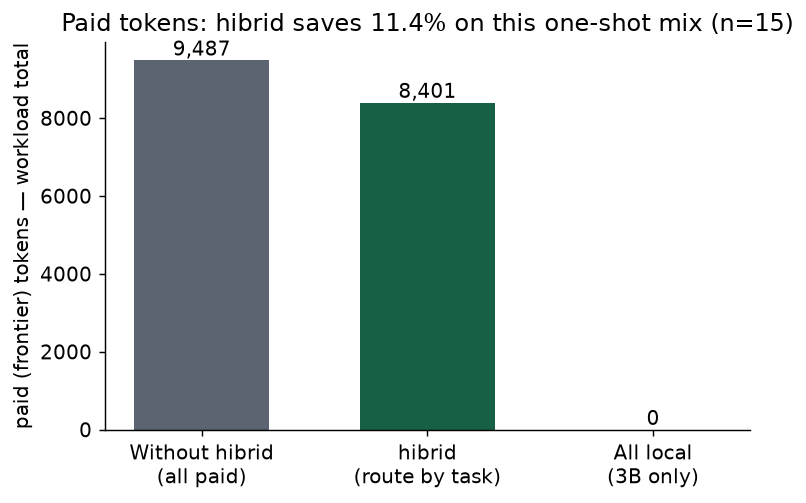
\includegraphics[width=0.62\textwidth]{eval_tokens.png}
\end{center}
\caption{Paid (frontier) tokens over the judged workload ($n{=}15$): all-paid 9{,}487 vs.\ 8{,}401 with difficulty-aware routing ($-11.4\%$) vs.\ 0 all-local. Hard tasks dominate token volume in this one-shot mix.}
\label{fig:tokens}
\end{figure}

\subsection{RQ4 --- Cost/quality}
\label{sec:rq4}

Figure~\ref{fig:pareto} plots the three operating points ($n{=}15$): \textsc{all-local} at $(0~\mathrm{tokens},\, Q\,0.631)$, \emph{difficulty-aware routing} at $(8{,}401,\, Q\,0.887)$ --- \textbf{92.9\%} of all-paid quality --- and \textsc{all-frontier} at $(9{,}487,\, Q\,0.955)$. Going fully local buys 100\% of the token bill for a 34\% quality drop --- acceptable only for trivial traffic. The routed point is the interesting one: giving up 6.8 points of quality ($0.955 \to 0.887$) saves 11.4\% of the bill on this mix, and the same policy scales its savings with the trivial share of real traffic (42--87.5\% in the agent-session studies above).

\begin{figure}[t]
\begin{center}
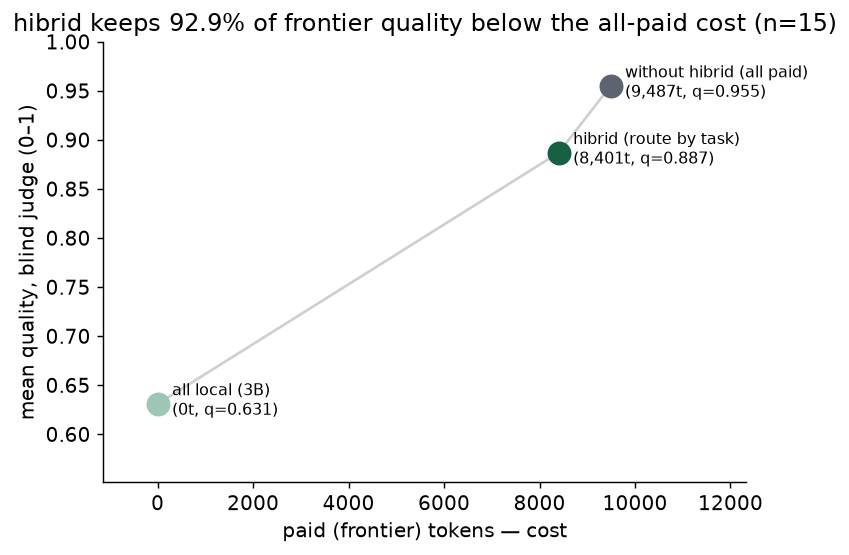
\includegraphics[width=0.66\textwidth]{eval_pareto.png}
\end{center}
\caption{Cost/quality plane ($n{=}15$). Difficulty-aware routing keeps 92.9\% of all-paid quality below the all-paid cost; all-local is free but drops to $Q\,0.631$.}
\label{fig:pareto}
\end{figure}

\subsection{RQ5 --- Positioning}
\label{sec:rq5}

Figure~\ref{fig:competitors} places hibrid's differentiators (local-first, no API key, hardware-aware, open-source) against reported competitor savings. We stress that the competitor bars are \emph{reported under their authors' own conditions and are not comparable} to our measured numbers; the figure is a map of the landscape, not a head-to-head. RouteLLM's reported ``95\% of GPT-4 quality at 74--86\% saving'' uses a \emph{trained} router over a large preference dataset; our measured 92.9\%/11.4\% point uses a heuristic difficulty split on a deliberately hostile hardware floor --- the gap is the price of not having a learned router yet.

\begin{figure}[t]
\begin{center}
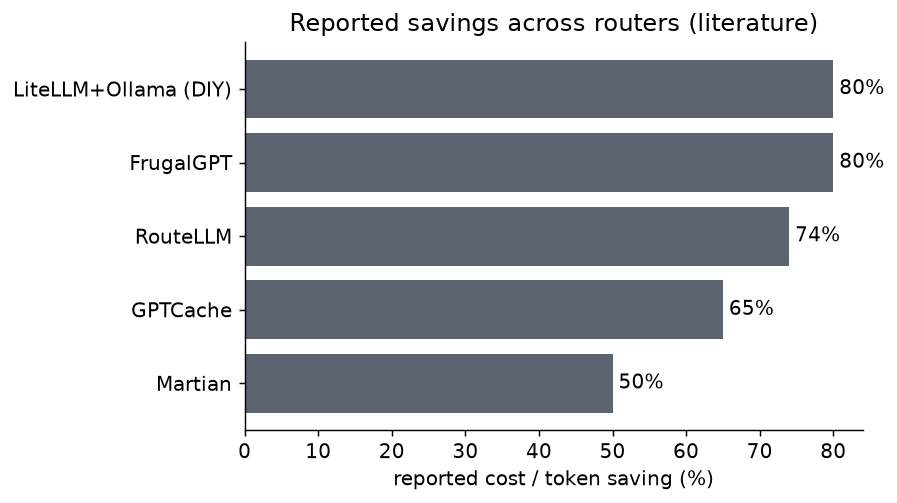
\includegraphics[width=0.7\textwidth]{eval_competitors.png}
\end{center}
\caption{Reported cost/token savings across routers (authors' own conditions; not comparable). hibrid's numbers are measured in this paper (Figures~\ref{fig:tokens} and \ref{fig:pareto}), not reported.}
\label{fig:competitors}
\end{figure}

\section{Discussion}
\label{sec:discussion}

Three findings survive the corrected data. \textbf{First}, a 3B model on a CPU node keeps ${\sim}87\%$ of frontier quality on trivial tasks and reaches parity on a quarter of the battery --- the free tier is genuinely useful, but only there. \textbf{Second}, the frontier earns its cost exactly where the router should send it: hard reasoning ($0.398$ vs.\ $0.965$ is the largest gap we measured). \textbf{Third}, token savings depend on workload shape: $-11.4\%$ on a hard-heavy one-shot mix, $-87.5\%$ on a loop-heavy agent session. A router pitch quoting only the second number would be dishonest; quoting only the first would undersell the mechanism.

The live engine currently escalates by \emph{local adequacy and latency} rather than a learned hardness signal: on a capable node it keeps everything local (the sweep), on a weak node it escalates broadly (15/16). That is safe --- it never ships an unusably slow local answer --- but coarse: it spent paid-cheap tokens on trivial tasks the 3B model handles at 86.8\% quality. A difficulty or hardness signal, even the heuristic one evaluated in \S\ref{sec:rq4}, is the single highest-value improvement.

\section{Limitations and Future Work}
\label{sec:limitations}

\textbf{Judge validity.} A single frontier judge ($N{=}1$, one pass) scored answers; no inter-judge agreement was computed, and the judge shares a model family with the frontier answers, risking self-preference despite blinding and randomised order. One task was lost to judge JSON parsing ($n{=}15$).
\textbf{Statistical power.} $n{=}15$; per-axis cells are 2--4 tasks --- indicative, not powered. No confidence intervals are claimed. The battery is small and hand-written; real traffic differs.
\textbf{Single node, single small model.} Quality was measured with one ${\sim}$3B-class local setup on one CPU node; stronger local models on GPU or Apple-silicon nodes should narrow the trivial-task gap and may narrow the hard-task gap. One local row used \texttt{qwen2.5-coder:1.5b} (the local tier's own model choice); we report it as measured.
\textbf{Policy vs.\ product.} The difficulty-aware routing point (\S\ref{sec:rq4}) uses the battery's ground-truth difficulty labels, i.e.\ an oracle split; the shipped router does not yet infer hardness. The live-engine numbers (15/16 escalated) are the product today; the routed point is its target.
\textbf{Comparability.} All competitor numbers are reported by their authors; we did not re-run them.
\textbf{Future work:} a learned or output-aware escalation signal; multi-judge scoring with agreement statistics; a larger battery; submission to RouterBench/LLMRouterBench for independent replication.

\section{Conclusion}
\label{sec:conclusion}

\textbf{RQ1:} routing decisions are correct (197/197 assertions at zero token cost). \textbf{RQ3:} a 3B local model on a worst-case node retains \textbf{66\%} of frontier quality overall --- \textbf{87\%} on trivial tasks, \textbf{42\%} on hard ones, with hard reasoning as the decisive gap. \textbf{RQ2/RQ4:} difficulty-aware routing keeps \textbf{92.9\%} of all-frontier quality while cutting paid tokens by \textbf{11.4\%} on this one-shot mix, and by up to \textbf{87.5\%} on loop-heavy agent sessions where cheap calls dominate. \textbf{RQ5:} hibrid uniquely combines local-first, no-API-key, hardware-aware routing, but lacks a trained router and independent benchmarking. The honest summary: \emph{the small model is not the product --- the split is.}

\subsubsection*{Broader Impact Statement}
Local-first routing reduces the marginal cost of LLM inference and keeps private data on the user's machine by default, which we view as positive for access and privacy. The main risk is over-trusting small-model output on tasks that look trivial but are not; the measured hard-task gap (42.5\% retained) quantifies exactly that risk, and the router's conservative escalation is designed to mitigate it.

\subsubsection*{Author Note: An AI-Made Paper}
This evaluation --- harness code, experiment execution, statistical analysis, figures, and the text of this paper --- was produced by AI agents operating the hibrid project, with a human owner supervising scope and auditing results (including catching an earlier contaminated run, \S\ref{sec:intro}). We disclose this so readers can weigh the evidence accordingly; all raw data and code needed to check every number are public in the artifact.

\subsubsection*{Reproducibility Statement}
The artifact (\url{https://github.com/vfalbor/hibrid}) contains the harness, the versioned 16-prompt battery, raw per-task results (answers, tokens, tiers, scores, judge rationales), the routing sweep, and the scripts that regenerate every figure and statistic in this paper from the raw results file:
\begin{verbatim}
python tests/batch_qa.py                     # RQ1: decision battery, 0 tokens
python docs/benchmarks/eval_run.py           # RQ2-RQ4: provenance-checked run
python docs/benchmarks/eval_routing_sweep.py # RQ2: FTA across hardware tiers
python docs/benchmarks/eval_charts.py        # Figures 2-5 from raw results
\end{verbatim}
The judge ran blind with randomised answer order (fixed seed). The harness aborts if any frontier row is not \texttt{tier=paid\_strong}.

\bibliography{refs}
\bibliographystyle{tmlr}

\end{document}
